\documentclass{standalone}
\usepackage{tikz}
\begin{document}
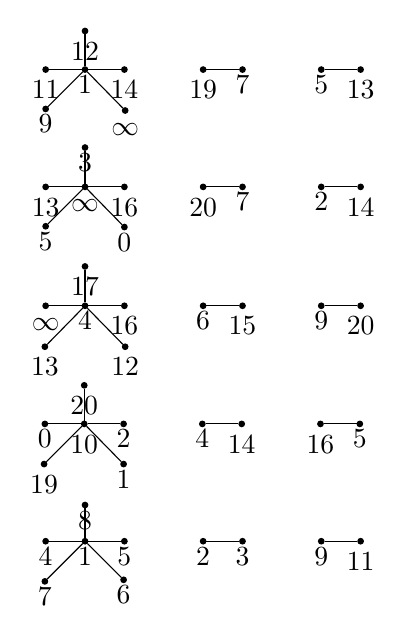
\begin{tikzpicture}[every node/.style={draw, circle, fill=black, minimum size=2pt, inner sep=0pt}]
\node[fill=black, label=below:{\color{black}$11$}] (G1N11) at (4.00,7.00) {};
\node[fill=black, label=below:{\color{black}$1$}] (G1N1) at (4.50,7.00) {};
\node[fill=black, label=below:{\color{black}$14$}] (G1N14) at (5.00,7.00) {};
\node[fill=black, label=below:{\color{black}$\infty$}] (G1Ninf) at (5.01,6.48) {};
\node[fill=black, label=below:{\color{black}$9$}] (G1N9) at (4.00,6.50) {};
\node[fill=black, label=below:{\color{black}$12$}] (G1N12) at (4.50,7.49) {};
\node[fill=black, label=below:{\color{black}$19$}] (G1N19) at (6.00,7.00) {};
\node[fill=black, label=below:{\color{black}$7$}] (G1N7) at (6.50,7.00) {};
\node[fill=black, label=below:{\color{black}$5$}] (G1N5) at (7.50,7.00) {};
\node[fill=black, label=below:{\color{black}$13$}] (G1N13) at (8.00,7.00) {};
\draw (G1N1) -- (G1N11);
\draw (G1N1) -- (G1N14);
\draw (G1N1) -- (G1Ninf);
\draw (G1N1) -- (G1N9);
\draw (G1N1) -- (G1N12);
\draw (G1N7) -- (G1N19);
\draw (G1N5) -- (G1N13);
\node[fill=black, label=below:{\color{black}$13$}] (G2N13) at (4.00,5.51) {};
\node[fill=black, label=below:{\color{black}$\infty$}] (G2Ninf) at (4.50,5.51) {};
\node[fill=black, label=below:{\color{black}$16$}] (G2N16) at (5.00,5.51) {};
\node[fill=black, label=below:{\color{black}$0$}] (G2N0) at (5.00,5.00) {};
\node[fill=black, label=below:{\color{black}$5$}] (G2N5) at (4.00,5.01) {};
\node[fill=black, label=below:{\color{black}$3$}] (G2N3) at (4.50,6.01) {};
\node[fill=black, label=below:{\color{black}$20$}] (G2N20) at (6.00,5.51) {};
\node[fill=black, label=below:{\color{black}$7$}] (G2N7) at (6.50,5.51) {};
\node[fill=black, label=below:{\color{black}$2$}] (G2N2) at (7.50,5.51) {};
\node[fill=black, label=below:{\color{black}$14$}] (G2N14) at (8.00,5.51) {};
\draw (G2Ninf) -- (G2N13);
\draw (G2Ninf) -- (G2N16);
\draw (G2Ninf) -- (G2N0);
\draw (G2Ninf) -- (G2N5);
\draw (G2Ninf) -- (G2N3);
\draw (G2N7) -- (G2N20);
\draw (G2N2) -- (G2N14);
\node[fill=black, label=below:{\color{black}$\infty$}] (G3Ninf) at (4.00,4.00) {};
\node[fill=black, label=below:{\color{black}$4$}] (G3N4) at (4.50,4.00) {};
\node[fill=black, label=below:{\color{black}$16$}] (G3N16) at (5.00,4.00) {};
\node[fill=black, label=below:{\color{black}$12$}] (G3N12) at (5.01,3.48) {};
\node[fill=black, label=below:{\color{black}$13$}] (G3N13) at (3.99,3.48) {};
\node[fill=black, label=below:{\color{black}$17$}] (G3N17) at (4.50,4.50) {};
\node[fill=black, label=below:{\color{black}$6$}] (G3N6) at (6.00,4.00) {};
\node[fill=black, label=below:{\color{black}$15$}] (G3N15) at (6.50,4.00) {};
\node[fill=black, label=below:{\color{black}$9$}] (G3N9) at (7.50,4.00) {};
\node[fill=black, label=below:{\color{black}$20$}] (G3N20) at (8.00,4.00) {};
\draw (G3N4) -- (G3Ninf);
\draw (G3N4) -- (G3N16);
\draw (G3N4) -- (G3N12);
\draw (G3N4) -- (G3N13);
\draw (G3N4) -- (G3N17);
\draw (G3N6) -- (G3N15);
\draw (G3N9) -- (G3N20);
\node[fill=black, label=below:{\color{black}$0$}] (G4N0) at (3.99,2.50) {};
\node[fill=black, label=below:{\color{black}$10$}] (G4N10) at (4.49,2.50) {};
\node[fill=black, label=below:{\color{black}$2$}] (G4N2) at (4.99,2.50) {};
\node[fill=black, label=below:{\color{black}$1$}] (G4N1) at (4.99,1.99) {};
\node[fill=black, label=below:{\color{black}$19$}] (G4N19) at (3.98,1.99) {};
\node[fill=black, label=below:{\color{black}$20$}] (G4N20) at (4.49,2.99) {};
\node[fill=black, label=below:{\color{black}$4$}] (G4N4) at (5.99,2.50) {};
\node[fill=black, label=below:{\color{black}$14$}] (G4N14) at (6.49,2.50) {};
\node[fill=black, label=below:{\color{black}$16$}] (G4N16) at (7.49,2.50) {};
\node[fill=black, label=below:{\color{black}$5$}] (G4N5) at (7.99,2.50) {};
\draw (G4N10) -- (G4N0);
\draw (G4N10) -- (G4N2);
\draw (G4N10) -- (G4N1);
\draw (G4N10) -- (G4N19);
\draw (G4N10) -- (G4N20);
\draw (G4N4) -- (G4N14);
\draw (G4N5) -- (G4N16);
\node[fill=black, label=below:{\color{black}$4$}] (G5N4) at (4.00,1.01) {};
\node[fill=black, label=below:{\color{black}$1$}] (G5N1) at (4.50,1.01) {};
\node[fill=black, label=below:{\color{black}$5$}] (G5N5) at (5.00,1.01) {};
\node[fill=black, label=below:{\color{black}$6$}] (G5N6) at (4.99,0.52) {};
\node[fill=black, label=below:{\color{black}$7$}] (G5N7) at (3.99,0.50) {};
\node[fill=black, label=below:{\color{black}$8$}] (G5N8) at (4.50,1.47) {};
\node[fill=black, label=below:{\color{black}$2$}] (G5N2) at (6.00,1.01) {};
\node[fill=black, label=below:{\color{black}$3$}] (G5N3) at (6.50,1.01) {};
\node[fill=black, label=below:{\color{black}$9$}] (G5N9) at (7.50,1.01) {};
\node[fill=black, label=below:{\color{black}$11$}] (G5N11) at (8.00,1.01) {};
\draw (G5N1) -- (G5N4);
\draw (G5N1) -- (G5N5);
\draw (G5N1) -- (G5N6);
\draw (G5N1) -- (G5N7);
\draw (G5N1) -- (G5N8);
\draw (G5N2) -- (G5N3);
\draw (G5N9) -- (G5N11);
\end{tikzpicture}
\end{document}
